\documentclass[12pt]{article}
%\renewcommand\normalsize{\fontsize{10pt}{12pt}\selectfont}
\usepackage{graphicx} % Required for inserting images
\usepackage[left=2cm,right=2cm,top=2cm,bottom=1.5cm]{geometry}

\title{HW 1}
%\author{Dennis Wilkinson}
%\date{March 31 2025; due Monday April 7}

\begin{document}

\setlength{\parindent}{0pt}
\setlength{\parskip}{3mm}




%\maketitle

FS1 Wilkinson

HW 1, March 31, 2025; due April 7


1. A student walks north on Congress Ave starting at 2nd St. For one block he walks at a typical speed. He stops and waits 6 seconds for a traffic light to change. He then continues walking north one more block at variable speed while doing really important things on his phone. At the next light, he sprints backward half a block to retrieve the homework papers he dropped. After retrieving the papers, being almost late, he jogs north all the way to 6th street. 

a. Plot his trip on $x$ vs $t$ and on $v$ vs $t$ axes (make two separate plots). Use reasonably accurate values for the length of a block (they can all be equal) and running/walking speeds. Use meters for length and label your axes.

b. Label the point where his speed - meaning, the rate at which his position changed - was maximum, on both plots.

c. What was his average speed for this trip?

d. Make a plot of $a$ vs $t$ for the trip. This one can be qualitative - no precise numbers required. 

%\bigskip
%\parskip{5mm}
\bigskip

\bigskip

\bigskip


2. At time $t=0$, a car accelerates forward from rest at a rate of $a$ meters per second squared. 

a. After $t$ seconds, show that the car's speed is $at$. If this is confusing, try putting in some numbers.

b. Plot the car's speed vs time graph. 

c. The distance covered by the car from 0 until $t$ is the area under the $v$ curve from 0 to $t$. Explain why.

d. Using geometry, calculate the area of this triangle and show that it equals $\frac{1}{2}at^2$.

e. If the car had an initial speed of $v_0$ instead of 0, but still accelerated at the rate $a$ starting at $t=0$, show (again using geometry) that the area under the curve is now $v_0t+\frac{1}{2}at^2.$ You should probably redo the plot in part c. 

f*. The car's motion is described by $\frac{d^2x}{dt^2}=a$ where $a$ is a constant. Solve this with initial conditions $x(0)=0$ and $v(0)=v_0$ to get the same result as in part e (equivalently, show that the result of part (e) satisfies $\frac{d^2x}{dt^2}=a$ with the correct initial conditions). Remember that $v=\frac{dx}{dt}.$

g. Solve this using the equation from part e: A Tesla is sitting at a traffic light. At time $t=0$ the light turns green and a VW Beetle, whose driver timed the light perfectly, zips past, hitting the intersection at 12 m/s and accelerating from there. The Tesla accelerates at 9 m/$s^2$ while the VW manages only 4 m/$s^2$. After 4 seconds, how far has each traveled, and who is ahead? Is either car speeding, if the road is Congress Ave?

\newpage

3. A ball is tossed in the air and is then is caught. A motion detector registers its speed and position during this process. The software produces the following plots of $x$ vs $t$ and $v$ vs $t$, respectively (position first) for the ball's motion.

%\begin{figure}
 %   \centering
    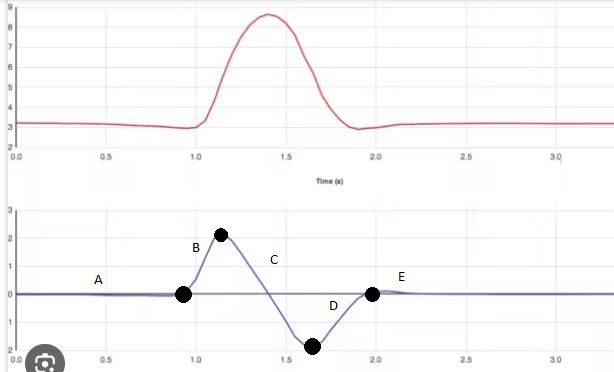
\includegraphics[width=0.9\linewidth]{Capture.JPG}
  %  \caption{Enter Caption}
   % \label{fig:enter-label}
%\end{figure}


a. Use the plots to show that the instantaneous speed is zero when the ball is at the top of its arc.

b. Looking at the $v$ vs $t$ graph, let's split the data into five sections, (A)-(E) as delineated by the dots in the graph.

For each section, which direction is the acceleration (or is it zero), and is it constant or changing? Use the slope of the $v$ curve and not necessarily your intuition.

c. What was happening in each section? You need to explain sections B and D particularly.

d. Calculate the approximate acceleration in section C, using the numbers on the graph.

\newpage

4. A pendulum is swinging back and forth and the motion detector makes the following plots.

%\begin{figure}
%    \centering
    %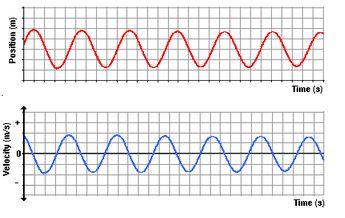
\includegraphics[width=0.5\linewidth]{C3.JPG}
%\end{figure}
%\begin{figure}
    %\centering
    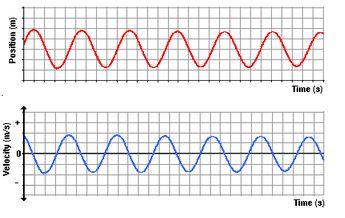
\includegraphics[width=0.5\linewidth]{C3.JPG}
 %   \caption{Enter Caption}
  %  \label{fig:enter-label}
%\end{figure}

a. Pick a moment when the position is zero (middle of the motion). What is the velocity at this moment? What about the acceleration (slope of $v$)?

b. Pick a moment when the velocity is zero. What is the position at this moment - min, max, zero, something else? What about the acceleration? 

c. This is an example of an object whose velocity is zero when its acceleration is not zero. Can you think of another example?

d*. The pendulum motion is best described by considering the angle $\theta$ that the string makes with the vertical. In this case, the motion is determined by the equation $\frac{d^2\theta}{dt^2}=-\frac{g}{l}\sin\theta$, where $l$ is the pendulum length and $g$ is the acceleration of gravity. Usually, at this point, people assume $\theta$ is small, so that $\sin\theta \approx \theta$ and the motion equation becomes $\frac{d^2\theta}{dt^2}=-\frac{g}{l}\theta$. 

Show that one possible solution in this case is $\theta(t)=\frac{\pi}{6}\cos\omega t$, where $\omega=\sqrt{\frac{g}{l}}$. What is the initial value $\theta_0$ at time $t=0$ in this case? This value is in radians.

e. Show that with the solution of part d, the period $T$, which is the time it takes the pendulum to make one full swing, equals $2\pi\sqrt{\frac{l}{g}}$. 

f*.  If we don't make the approximation of small $\theta$, the pendulum equation does not have a solution in the form of elementary equations (sine, cosine, exponential, etc). Instead, after some little algebra, we can find that the period is given by $T=4\sqrt{\frac{l}{g}}K(k)$, where $k=\sin\frac{\theta_0}{2}$ and $K$ is a special function called the "complete elliptical integral of the 1st kind" which equals $\int_0^{\pi/2}\frac{dx}{\sqrt{1-k^2\sin^2x}}$. Using mathematical software or online resources, calculate the period for the initial condition that you calculated in part d. What percentage error would we make by using the small angle approximation (formula in part e) to calculate T? What is the percent error if the initial angle is 8 degrees?


\end{document}
